\chapter{Sprawdzenie mo�liwo�� sterowania i pomiaru oraz wyznaczenie punktu pracy}

\section{Przyk�adowe sterowanie wraz z odczytem pomiar�w}

Podczas testu b�dziemy zmienia� sygna�y steruj�ce w nast�puj�cy spos�b:

\begin{align*} 
G1 = 100 \land G2 = 0 & \textrm{, dla } k \in <0, 10) \\ 
G1 = 100 \land G2 = 100 & \textrm{, dla } k \in <10, 50) \\
G1 = 20 \land G2 = 20 & \textrm{, dla } k \in <50, 100) \\
G1 = 25 \land G2 = 15 & \textrm{, dla } k \geqslant 100
\end{align*}

\begin{figure}
	\centering
	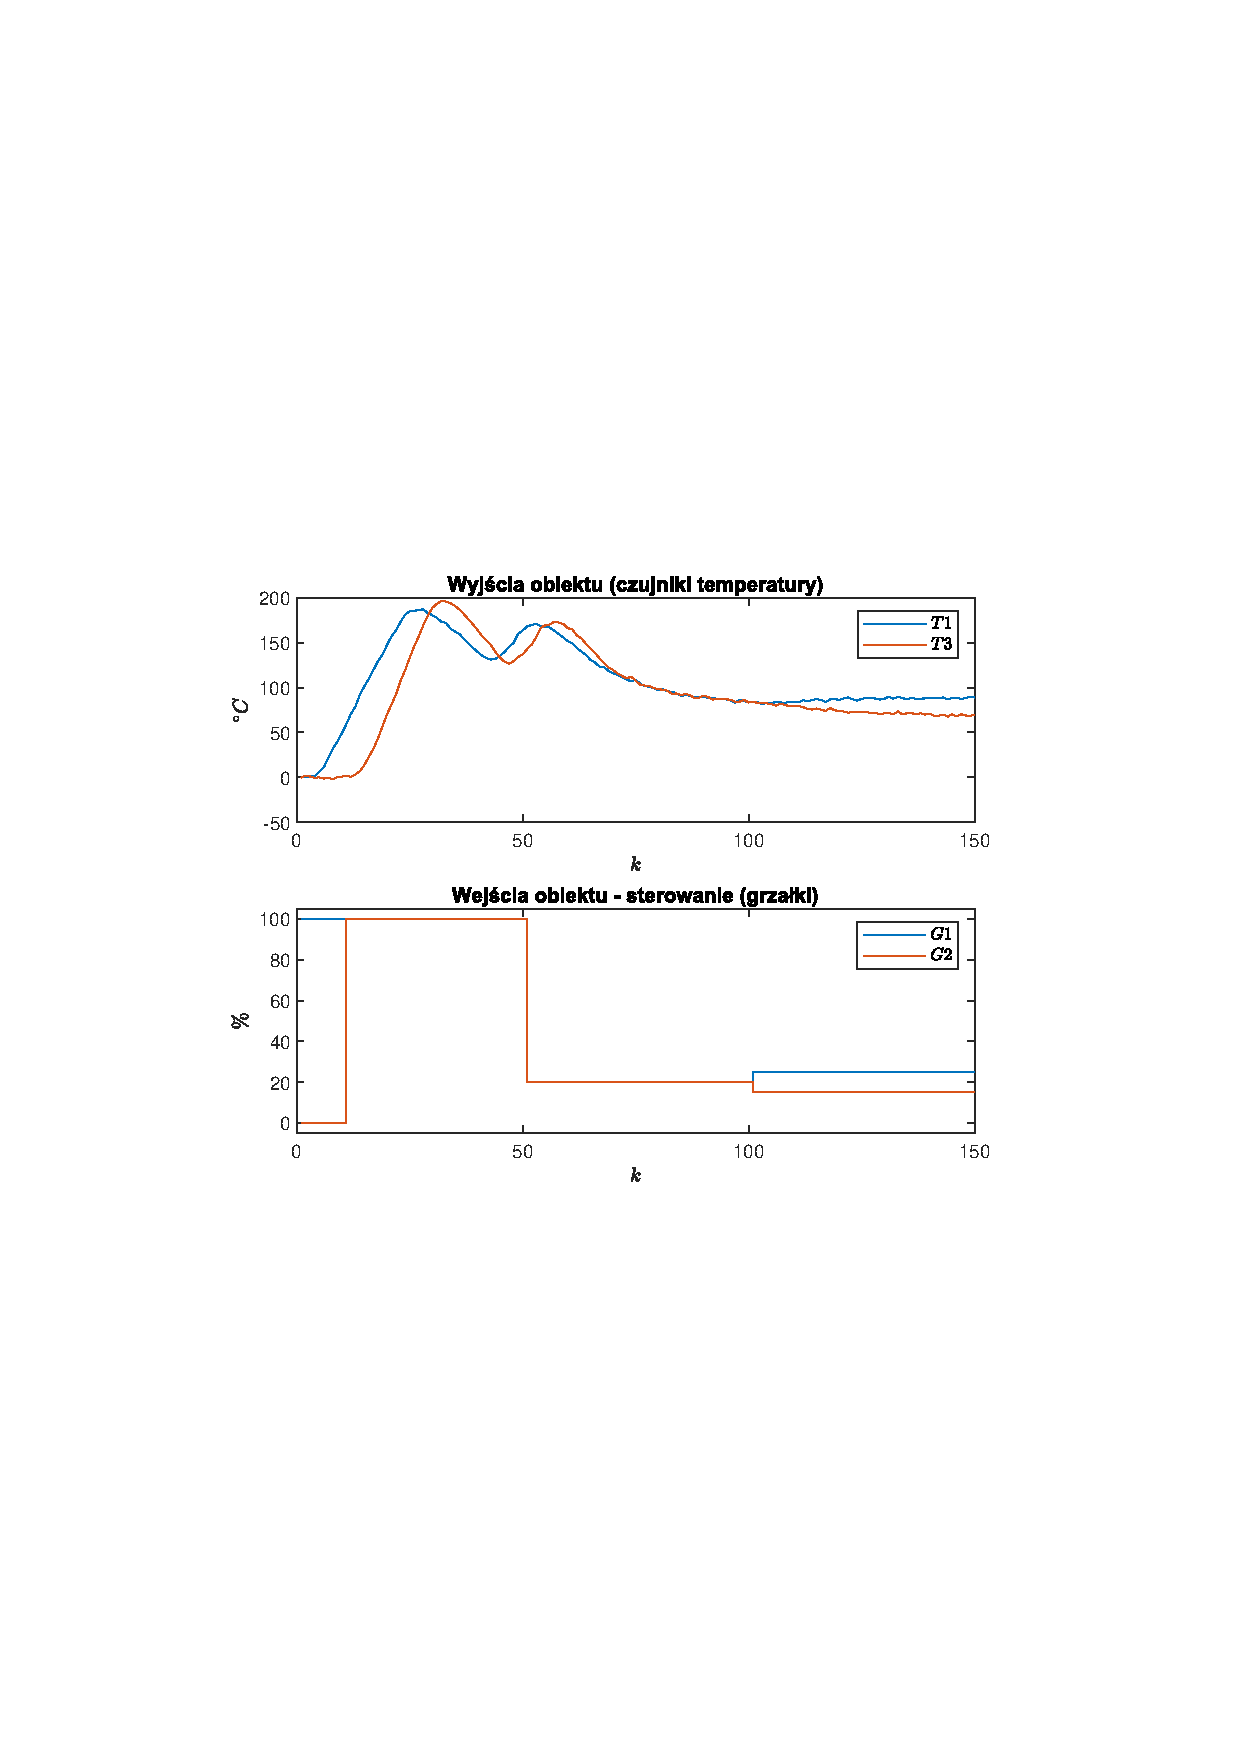
\includegraphics[scale=0.85, trim={2cm 8.5cm 2cm 8.5cm}]{rysunki/test}
	\caption{Sprawdzenie mo�liwo�� sterowania i pomiaru w komunikacji ze stanowiskiem}
	\label{test}
\end{figure}

Jak widzimy mamy mo�liwo�� sterowania i pomiaru w komunikacji ze stanowiskiem.

\subsection{Implementacja}

Do przetestowania mo�liwo�ci sterowania i pomiaru w komunikacji ze stanowiskiem u�yto skryptu \verb+zad1_1.m+.

\section{Punkt pracy}

Jako punkt pracy wybrali�my: $G1 = \num{18}$, $G2 = \num{23}$.

\begin{figure}
	\centering
	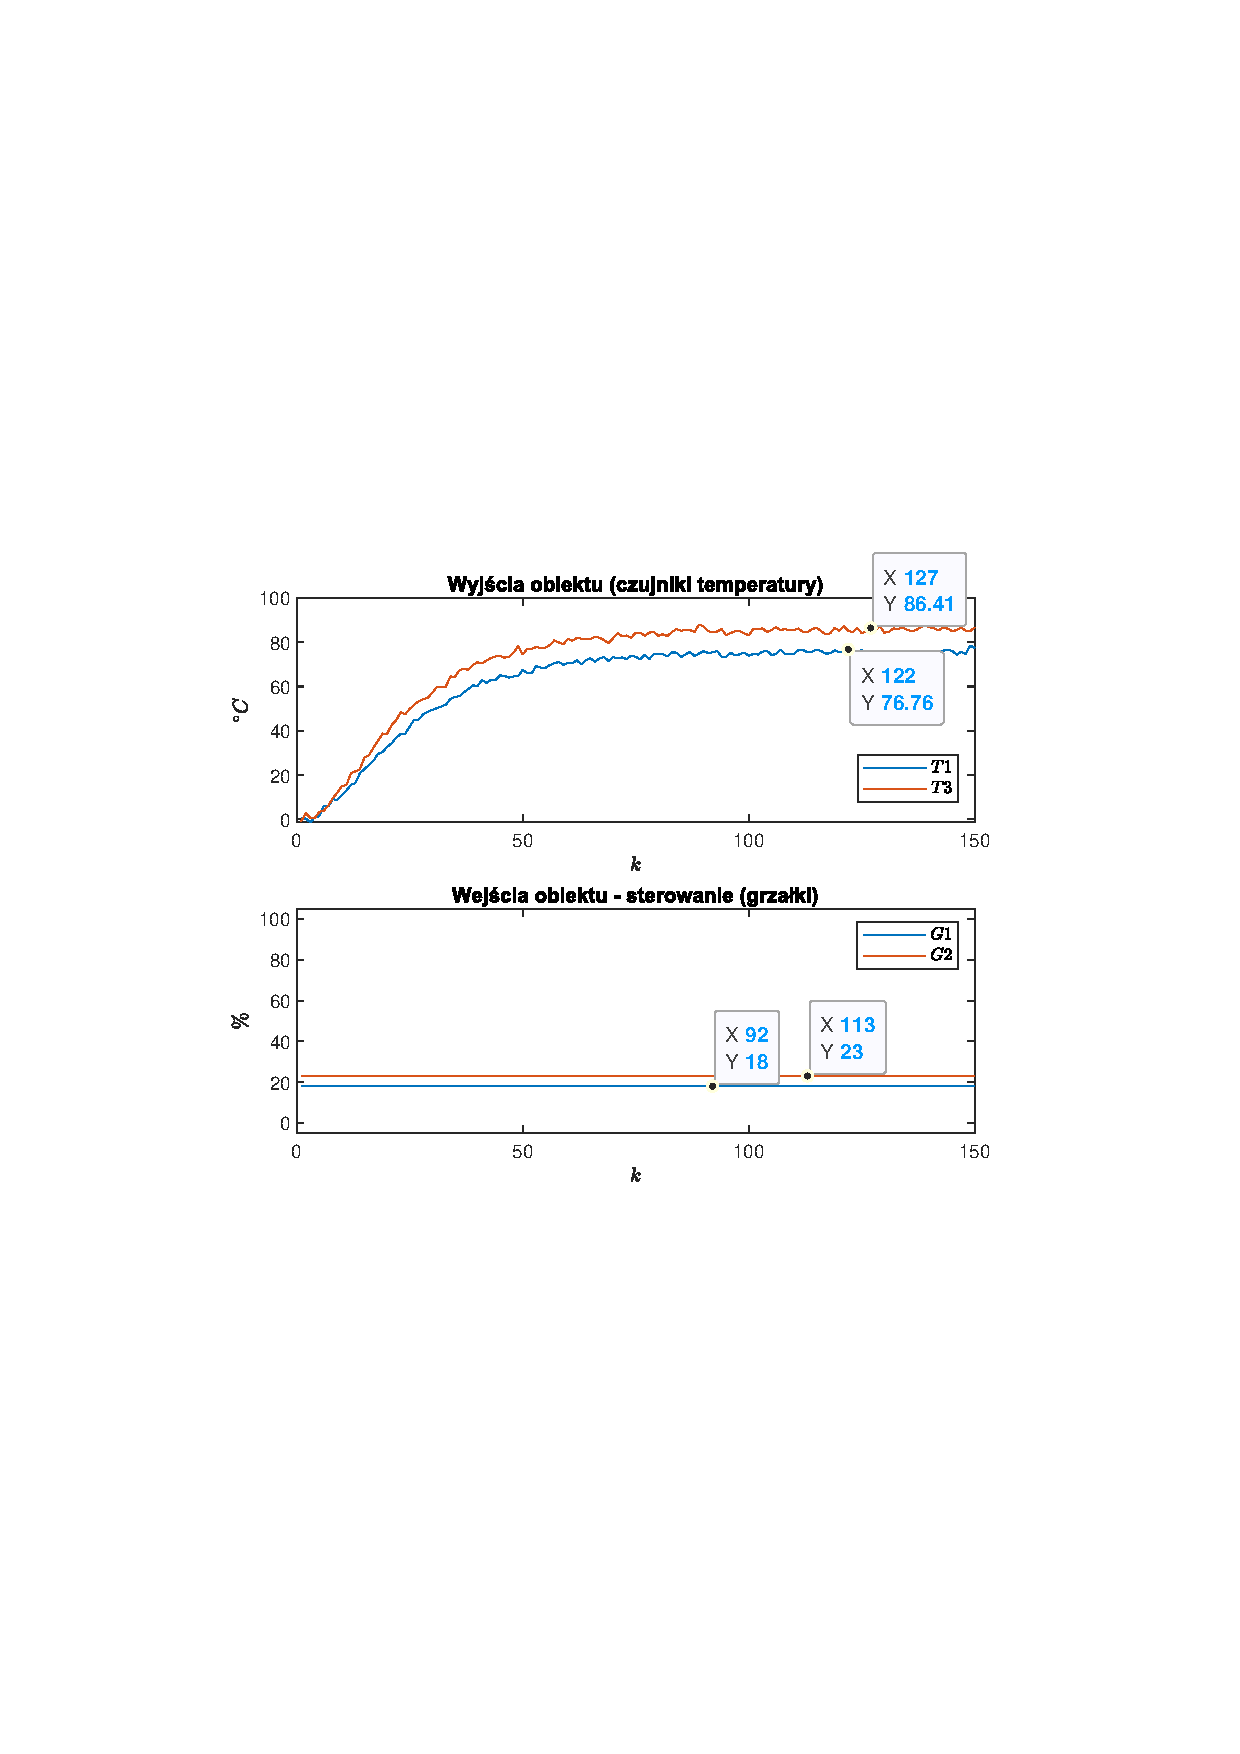
\includegraphics[scale=0.85, trim={2cm 8.5cm 2cm 8.5cm}]{rysunki/punkt_pracy}
	\caption{Punkt pracy}
	\label{punkt_pracy}
\end{figure}

Dla powy�szego punktu pracy pomiary z czujnik�w wynosz�: $T1 = \num{75.43}$, $T3 = \num{84.64}$.

\subsection{Implementacja}

Do wyznaczenia warto�ci temperatury, odczytanej z czujnika, wykorzystano skrypt \verb+zad1_2.m+.